\chapter{二元调制多符号条件归零接收机}
在上一章,我们系统讨论了高阶调制QAM信号的接收方案,
至此,常见的调制方案都已被比较系统的研究。
在这些方案中,通常都是针对单个符号设计的接收方案,
而正如第二章所述,采用针对编码后的多个符号设计的联合检测方案才有可能
逼近Holevo容量。因此这一章我们来讨论最简单的三种
调制方案的一种联合检测方案——条件归零接收机。


\section{MPPM信号条件归零接收机}
首先,我们来考虑一种特殊的编码方案,多脉冲脉冲位置调制(MPPM)信号。
与PPM信号的思想一样,信息被调制在脉冲的位置上面,
具有很高的能量效率,这在深空通信中具有潜在的应用价值\cite{hemmati2006deep}。
与PPM信号不同的是,它的每一个符号通常采用两个或者两个以上的脉冲
来加载信息。采用这种方式,
可以在保证的较高能量效率的同时,
还能有效的克服PPM信号低频谱效率的缺点\cite{sugiyama1989mppm}。
这在深空通信如地月通信、卫星到卫星通信等场景
具有潜在的优势\cite{hemmati2006deep,waseda2011numerical}。

\subsection{MPPM信号标准量子极限}
首先,我们先来从数学上定义MPPM信号符号集合。
设每一个MPPM信号符号有$M$个时隙,对每一个符号,
都有$L$个时隙有脉冲,而其他$M-L$个时隙没有脉冲,
我们称这种MPPM信号为L-M-PPM信号,如图\ref{fig:MPPM-DD}(\textit{a})所示。
一般的,我们只考虑$L \ge 2$的情形,$L=1$时就退化为单脉冲PPM的情形。
容易知道,这样的L-M-PPM信号的符号集合个数为
\begin{equation}
\binom{M}{L} = \frac{M(M-1)\cdots(M-L+1)}{L!}.
\end{equation}
例如当$M=4, L=2$时,2-4-PPM信号有$\binom{4}{2}=6$个,如果用1代表
有脉冲,而用0代表没有脉冲,那么这些信号可以编码为二进制码字
$\bm{c} = (c_1, c_2, \cdots, c_M)$,对2-4-PPM信号这6个码字为
\begin{equation}
\begin{array}{cccc}
1 & 0 & 0 & 1 \\
1 & 0 & 1 & 0 \\
1 & 1 & 0 & 0 \\
0 & 1 & 0 & 1 \\
0 & 1 & 1 & 0 \\
0 & 0 & 1 & 1   
\end{array}
\end{equation}
在将这些码字映射到量子态时,我们用相干态$\ket{0}$和$\ket{\alpha}$
分别代表0和1,用直积态
\begin{equation}
\ket{\gamma_1}\otimes\ket{\gamma_2}\otimes\cdots\otimes\ket{\gamma_M}, \\
\ket{\gamma_i} = \begin{cases}
                    \ket{0}, & c_i=0, \\
                    \ket{\alpha}, & c_i=1
                \end{cases}
\end{equation}
来表示每一个码字对应的信号。

\begin{figure}
\centering
  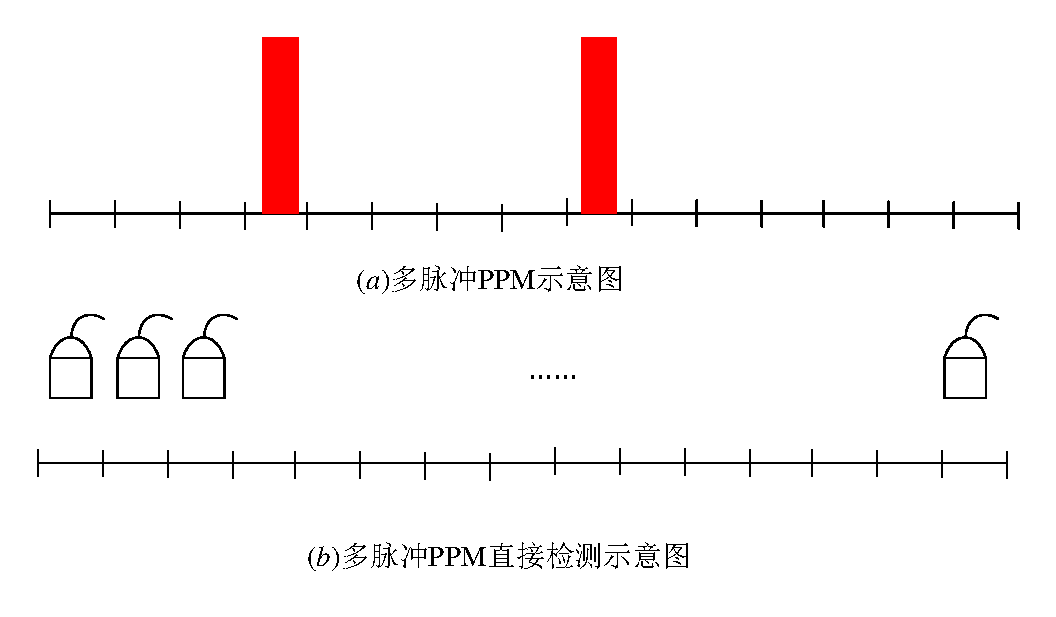
\includegraphics[width=0.8\textwidth]{figures/chap4/MPPM-DD}
  \caption{MPPM信号和直接检测示意图}
  \label{fig:MPPM-DD}
\end{figure}

在经典的光通信系统中,与PPM信号一样,采用直接检测的方法
对MPPM信号进行探测\cite{simon2003multi}。
直接检测探测方法利用一个ON-OFF探测器,
对每一个时隙进行独立的探测。
设每一个时隙的输出为$o_i$,如果有脉冲
$o_i=1$,否则$o_i=0$。
那么$M$个时隙对应的$M$个输出
构成输出序列$\bm{o} = (o_1,o_2,\cdots,o_M)$。
当所有的$M$个时隙都探测完毕,
然后通过最大似然准则进行译码判决\cite{simon2003multi}。
如果所有码字的先验概率是相同的(通信中通常都满足),这种判决准则使得平均错误概率最低。
对于给定的码字$\bm{c}_i$,输出序列为$\bm{o}$的条件概率为
\begin{equation}
\Pr{\bm{o} | \bm{c}_i} = \prod_{k=1}^M \left(1 - e^{-c_{ik}n} \right)^{o_{k}} \left(e^{-c_{ik}n} \right)^{1-o_{k}} .
\end{equation}
其中$\bm{c}_i=(c_{i1},\cdots,c_{iM})$
和$\bm{o}=(o_{1},\cdots,o_{M})$
分别为码字和输出序列,
$n=|\alpha|^2$是一个脉冲的平均光子数。
最大似然准则通过计算对给定的输出序列$\bm{o}$
每一个符号对应的条件概率,
选择出条件概率最大的符号进行判决,
该条件概率也称似然函数。

理想情况下,实际检测到脉冲数目$K \le L$,此时上述
条件概率也即是似然函数变为
\begin{equation}
\Lambda_i = \Pr{\bm{o} | \bm{c}_i} = \begin{cases} 
                                        \left(1 - e^{-n} \right)^{K} \left(e^{-n} \right)^{L-K}, & o_k \le c_{ik} \forall k,\\
                                        0,                                                       & \text{otherwise}.
                                    \end{cases}
\end{equation}
对于给定的码符号集合,$L$是相同的,
所以根据最大似然准则,对给定的输出序列$\bm{o}$,
只要满足$o_k \le c_{ik} \forall k$的码字对应的
似然函数是相同的。此时随机选择一个判决输出。
因此,对给定的码字$\bm{c}_i$,
在探测到$K$个光子时接收机正确探测的概率为
\begin{equation}
\Pr{\bm{c}_i | \bm{c}_i} = \frac{1}{\binom{M-K}{L-K}} \binom{L}{K} \left(1 - e^{-n} \right)^{K} \left(e^{-n} \right)^{L-K}.
\end{equation}
所以,这种检测方案的平均错误概率为
\begin{equation}
\begin{split}
P_e &= \frac{1}{\binom{M}{L}}\sum_{i=1}^{\binom{M}{L}} \sum_{K=0}^{L} \Pr{\bm{c}_i | \bm{c}_i, K}  \\
    &= \sum_{K=0}^{L} \frac{1}{\binom{M-K}{L-K}} \binom{L}{K} \left(1 - e^{-n} \right)^{K} \left(e^{-n} \right)^{L-K}.
\end{split}
\end{equation}
下面我们考虑大信号近似,即当$n \gg 1$时,可以忽略少检测到的脉冲数目大于1个的情况的概率,
即
\begin{equation}
\begin{split}
\Pr{\bm{c}_i | \bm{c}_i} &\approx (1-e^{-n})^L + \frac{L}{M-L+1} (1-e^{-n})^{L-1} e^{-n} \\
                            &\approx 1 - L\left(1 - \frac{1}{M-L+1} \right)e^{-n}.
\end{split}
\end{equation}
因此,这种检测方案的渐近性能为
\begin{equation}
\begin{split}
P_e & \approx L\left(1 - \frac{1}{M-L+1} \right)e^{-n} \\
    & = L\left(1 - \frac{1}{M-L+1} \right)e^{-|\alpha|^2}.
\end{split}
\end{equation}



\subsection{MPPM信号Helstrom极限}
一般而言,MPPM信号并不具有几何均匀对称性,
为了求得这种信号的最优量子检测的性能,
需要如QAM信号那样求解半正定规划问题\ref{eq:Hel-SDP}。
因此,我们需要得到密度矩阵。
与QAM信号不同的是,MPPM信号是直积态,
如果采用QAM信号那种将每一个时隙的信号在Fork态中展开,
然后截取长度为$l$的向量,那么要表达整个直积态信号,
所需要的向量维度为$l^M$,将随着时隙数目$M$指数增长,
这将为计算带来困难。
所以这里我们采用Smit正交化的方法\cite{lzw2010LA,zyh2007szjsff},
构造一组新的基向量$\ket{e_i}$。
为方便计,我们用矢量$\ket{\psi_i}$表示这$N = \binom{M}{L}$个直积态信号,
那么基向量$\ket{e_i}$可以表达为
\begin{equation}
\begin{split}
\ket{u_1} &= \ket{\psi_1}, \ket{e_1} = \frac{\ket{u_1}}{\sqrt{\bra{u_1}\ket{u_1}}}\\
\ket{u_2} &= \ket{\psi_2} - \bra{e_1}\ket{\psi_2}\ket{e_1}, \ket{e_2} = \frac{\ket{u_2}}{\sqrt{\bra{u_2}\ket{u_2}}}\\
          &\qquad\qquad \vdots \\
\ket{u_N} &= \ket{\psi_N} - \sum_{k=1}^{N-1} \bra{e_k}\ket{\psi_N}\ket{e_k}, \ket{e_k} = \frac{\ket{u_N}}{\sqrt{\bra{u_N}\ket{u_N}}}.
\end{split}
\end{equation}
设在该基向量上,$\ket{\psi_i} =\bm{c}_i = (c_{i1} \quad c_{i2} \dots c_{in})^T$,
那么有
\begin{equation}
\begin{split}
c_{11} &= 1, c_{1k}=0 \quad k>1; \\
c_{ii} &= \sqrt{G_{ii} - \sum_{k=1}^{i-1} |c_{ik}|^2 }, c_{ik}=0 \quad k>i, \\
c_{ij} &= \bra{e_j}\ket{\psi_i} \\
       &= \frac{1}{\sqrt{\bra{u_j}\ket{u_j}}} \left( \bra{\psi_j}\ket{\psi_i} - \sum_{k=1}^{j-1} \bra{\psi_j}\ket{e_k} \bra{e_k}\ket{\psi_i} \right)\\
       &= \frac{1}{c_{jj}} \left( G_{ji} - \sum_{k=1}^{j-1} c_{jk}^* c_{ik} \right), \quad j<i.
\end{split}
\end{equation}
这里$G_{ji}=\bra{\psi_j}\ket{\psi_i}$为Gram矩阵元素,
对L-M-PPM信号,
这里两个信号之间的内积为
\begin{equation}
\bra{\psi_j}\ket{\psi_i}=e^{-1/2 d(\bm{c}_i, \bm{c}_j)^2 n}
\end{equation}
这里$d(\bm{c}_i, \bm{c}_j)$这这两个码字的Hamming距离。
利用上述结果,可以得到密度矩阵为
\begin{equation}
\hat{\rho_i} = \ket{\psi_i}\bra{\psi_i} = \bm{c}_i \bm{c}_i^\dagger.
\end{equation}
这里$\bm{c}_i^\dagger$表示$\bm{c}_i$的共轭转置。
一旦将密度矩阵表达为有限维矩阵之后,就可以利用CVX工具箱\cite{cvx,gb08}进行数值求解了。

进一步,利用\ref{eq:Hel-SDP}式,
我们可以求得一个平均错误概率的近似上界。
我们接下来证明一般地,当信号光强很大时$n \gg 1$,
存在非负实数$A_i$使得下式成立
\begin{equation}
\begin{split}
c_{ii} & \ge 1 - A_i e^{-1/2 d_{\min} n}, \\
c_{ij} & \le A_i e^{-1/2 d_{\min} n}, i\neq j.
\end{split}
\end{equation}
其中$d_{\min} = \min_{i \neq j} d(\bm{c}_i , \bm{c}_j)$
是码符号集合的最小汉明距离,容易验证$G_{ij} \le e^{-1/2 d_{\min} n}$。

当$i=1$时,显然成立。
我们假设当$i\le m$时成立,那么当$i=m+1$时,
存在非负实数$A_1, ..., A_{m+1}$,当$n \gg 1$时,有
\begin{equation}
\begin{split}
c_{m+1,j} & \le \frac{G_{j,m+1}}{c_{jj}} \\
       & \le \frac{e^{-1/2 d_{\min} n}}{1 - A_j e^{-1/2 d_{\min} n}}   \\
       & \le e^{-1/2 d_{\min} n} \left(  1 + 2 A_j e^{-1/2 d_{\min} n} \right)  \\
       & \le A_{m+1} A_j e^{-1/2 d_{\min} n}. \\
c_{m+1,m+1} &\ge \sqrt{1 - \sum_{k=1}^{m} A_k e^{-1/2 d_{\min} n} } \\
            &\ge 1 - \frac{1}{2}\sum_{k=1}^{m} A_{m+1} e^{-1/2 d_{\min} n} \\
            &\ge 1 - A_{m+1} A_{m+1} e^{-1/2 d_{\min} n}.
\end{split}
\end{equation}
所以上述命题成立,根据式\ref{eq:Hel-SDP},可得
\begin{equation}
\begin{split}
X_{ii} = \bra{e_i} \hat{X} \ket{e_i} \ge \bra{e_i} \hat{\rho}_i' \ket{e_i} = \frac{1}{N} c_{ii}  .
\end{split}
\end{equation}
所以平均错误概率
\begin{equation}
\begin{split}
P_e &= 1 - \Tr(\hat{X}) =  1 - \sum_i X_{ii} \\
    &\le \frac{1}{N} \sum_i A_i e^{- d_{\min} n}.
\end{split}
\end{equation}
即最优量子检测具有不高于$e^{- d_{\min} n}$形式的渐近性能上界。
事实上,上述结论可以推广到任意量子态集合,
采用最优检测其平均错误概率的渐近性能上界不高于
$e^{-n_{\min}}$,其中$n_{\min} = \min_{ij} |\bra{\psi_i}\ket{\psi_j}|^2$。

利用平方根检测,我们可以得到MPPM大信号时精确渐近性能。
因为
\begin{equation}
\begin{split}
\hat{Z}^2_{ii} \approx \sum_{d=d_{\min}} e^{-1/2 d_{\min} n} = B_i e^{-1/2 d_{\min} n}.
\end{split}
\end{equation}
这里$Z = I -G$,
假定$n \gg 1$,略去高阶小量,其中$B_i$是与码字$\bm{c}_i$距离等于
最小距离码字的个数。
所以由\ref{eq:Gram-approx}式,我们有
\begin{equation}
\begin{split}
P_e &= 1 - \frac{1}{M} \sum_{i=1}^M (1 - \frac{1}{8} \hat{Z}^2_{ii})^2 \\
    &\approx \frac{1}{4M} \sum_{i=1}^M \hat{Z}^2_{ii} \\
    &\approx \frac{1}{4} \sum_i B_i e^{-d_{\min} n} \\
    &\approx \frac{1}{2} D e^{-d_{\min} n}.
\end{split}
\end{equation}
这里$D$是码间距离等于最小距离的码字对数。
例如,对单脉冲PPM信号,任意两个码字间距离都是最小距离2,
所以它的渐近误差性能为$\frac{M(M-1)}{4} e^{-2 n}$.



\subsection{MPPM条件归零接收机}
在第二章,我们简单地介绍了Dolinar在1982年提出的,
针对PPM信号设计的条件归零(CPN)接收机。
我们将该接收机推广到更一般的情况,
用来接收MPPM信号。


\begin{figure}
\centering
  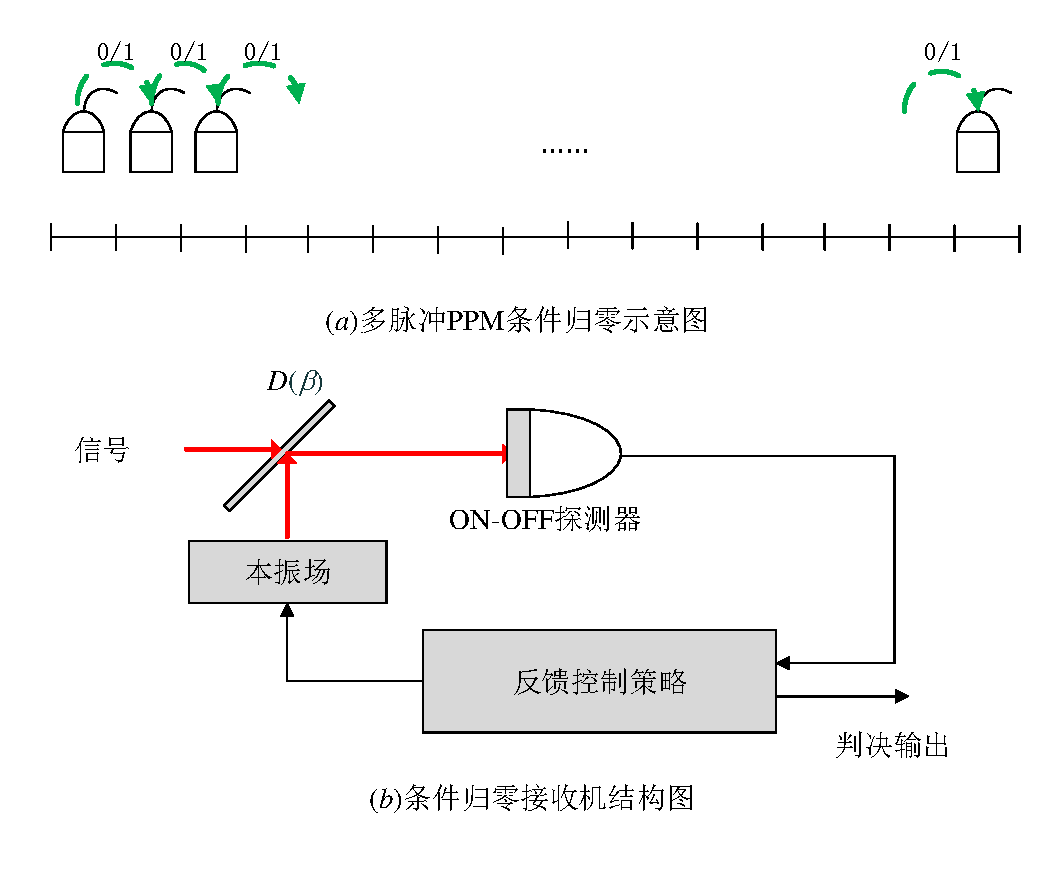
\includegraphics[width=0.8\textwidth]{figures/chap4/CPN}
  \caption{条件归零接收机及接收过程示意图}
  \label{fig:CPN}
\end{figure}

如图\ref{fig:CPN}所示,在每一个时隙,
信号通过一个高透过率分束器
与本振发生干涉,即对信号进行了位移操作,
对MPPM信号而言,位移操作被限定在$\hat{D}(0)$和$\hat{D}(-\alpha)$
中选择一个。
位移后的信号进入单光子探测器或者ON-OFF探测器,
它对应于一个二元POVM测量
\begin{equation}
\hat{\Pi}_0 = \ket{0}\bra{0}, \hat{\Pi}_1 = \hat{I} - \ket{0}\bra{0}.
\label{eq:ONOFF-POVM}
\end{equation}
如果采用$\hat{D}(0)$位移操作,即该时隙采用直接探测,我们记为A类探测,
那么
\begin{equation}
\begin{split}
p_{0|0} &= \Tr[\hat{\Pi}_0 \ket{0}\bra{0}] = 1,\\
p_{1|1} &= \Tr[\hat{\Pi}_1 \ket{\alpha}\bra{\alpha}] = 1-e^{-n}.
\end{split}
\label{eq:CPN-cond-1}
\end{equation}
这里$n=|\alpha|^2$是脉冲的平均光子数,
$p_{0|0}$代表信号在该时隙里没有光脉冲输出为0的条件概率,
$p_{1|1}$代表信号在该时隙里没有光脉冲输出为0的条件概率。
此时单个符号探测的平均错误概率为
\begin{equation}
P_e^{A} = p_1 e^{-n}.
\label{eq:DD-A-error}
\end{equation}
这里$p_1$代表有脉冲的先验概率。
如果采用$\hat{D}(-\alpha)$位移操作,即该时隙归零脉冲后再采用直接探测,我们记为B类探测,
那么
\begin{equation}
\begin{split}
p_{0|0} &= \Tr[\hat{\Pi}_0 \hat{D}(-\alpha)\ket{0}\bra{0}\hat{D}^\dagger(-\alpha)] = e^{-n},\\
p_{1|1} &= \Tr[\hat{\Pi}_1 \hat{D}(-\alpha)\ket{\alpha}\bra{\alpha}\hat{D}^\dagger(-\alpha)] = 0.
\end{split}
\label{eq:CPN-cond-2}
\end{equation}
此时单个符号探测的平均错误概率为
\begin{equation}
P_e^{B} = p_0 e^{-n}.
\label{eq:DD-B-error}
\end{equation}
这里$p_0$代表没有脉冲的先验概率。



反馈策略通过探测器接收到的历史结果和当前结果
来决定下一个时隙采用哪一种位移操作,
即下一个时隙的位移量可以表示为历史的输出和当前的输出的函数。
设当前时刻为$k$,历史输出为$\zeta_{k-1}=(z_1,z_2,...,z_{k-1})$,那么
下一时刻的位移量为
\begin{equation}
\beta_{k+1} = \beta_{k+1}([\zeta_{k-1} , z_k]) = \beta_{k+1}(\zeta_k).
\end{equation}
如果当前时刻的输出为$z_k=0$,即没有光子计数时间发生,
那么下一个时刻的位移量为$\beta([\zeta_{k-1} 0]) = \beta^{z_1...z_{k-1}0}$,
如果$z_k=1$,则$\beta([\zeta_{k-1} 1]) = \beta^{z_1...z_{k-1}1}$,
整个策略可以表示为一颗决策树如图\ref{fig:CPN-strategy}所示。



\begin{figure}
\centering
  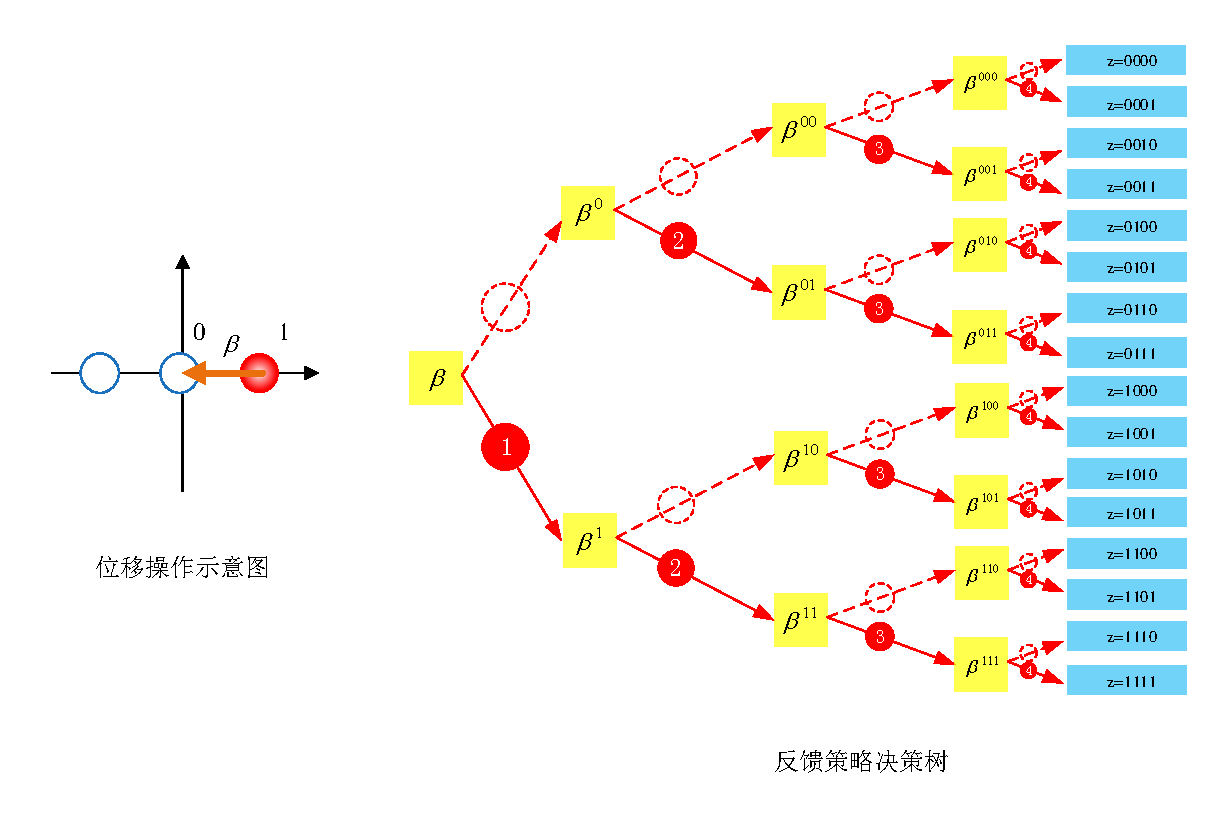
\includegraphics[width=\textwidth]{figures/chap4/CPN-strategy}
  \caption{条件归零接收机反馈策略决策树}
  \label{fig:CPN-strategy}
\end{figure}


当$M$个时隙都探测完毕,设探测器的输出序列为
$\bm{z}=[z_1,z_2,...,z_M]$,我们采用最大后验概率准则(MAP)进行判决,判决函数
\begin{equation}
h(\bm{z}) = \arg\max_i p_{i,\bm{z}}.
\end{equation}
这里$p_{i,\bm{z}}$代表发送第$i$个符号,同时输出序列为$\bm{z}$的联合概率。
那么对所有的符号,平均正确探测的概率为
\begin{equation}
P_c = \sum_z p_{h(\bm{z}),\bm{z}} = \sum_{\bm{z}} \max_i p_{i,\bm{z}}.
\end{equation}
当$M$个符号的先验概率一致时,最大后验概率准则与最大似然准则的结果一致。

现在,我们需要确定函数$\beta_k(\zeta_k)$的形式。
一种简单的取法是$\beta_k \equiv 0$,即每一个时隙都采用直接探测,
此时就是经典的检测方案。
通过观察\ref{eq:DD-A-error}式和\ref{eq:DD-B-error}式
我们可以知道$p_1 < p_0$时,即有脉冲的先验概率
比较大,适合采用B类探测,反之适合采用A类探测。
我们可以取位移策略为最大后验概率策略
\begin{equation}
\begin{split}
\beta_k(\zeta_{k-1}) &= \begin{cases}
                                0, & \text{符号} m_k^*(\zeta_{k-1}) \text{的第} k \text{个时隙没有脉冲}, \\
                                -\alpha, & \text{符号} m_k^*(\zeta_{k-1}) \text{的第} k \text{个时隙有脉冲}.
                             \end{cases} \\
m_k^*(\zeta_{k-1}) &=\arg\max_i p_{i,[z_1,...,z_{k-1}]}.   
\end{split}                          
\end{equation}

一般地,采用最大后验概率策略设计的反馈策略并不一定是最优策略。
为了得到最优策略,我们首先来定义优化目标函数\cite{dalla2014adaptive}
\begin{equation}
\begin{split}
J_k(s_k, \beta_{k+1}) & = \sum_{z' \in \mathcal{Z}_{M-K}} p_{h([\zeta_{k}, z']), [\zeta_{k}, z']}, (k=0,1,...,M-1) \\
J_{M}(s_{M}, \beta_{M+1}) & =  p_{h(\zeta_M), \zeta_M} = p_{h(\bm{z}), \bm{z}}.
\end{split}
\label{eq:reward-to-go-function}
\end{equation}
这里$s_k =s_k(\zeta_{k}) = [p_{1,\zeta_{k}},...,p_{M,\zeta_{k}} ]$是状态向量,
与前面的输出序列有关,
且初始状态$s_0 = [p_1,  ..., p_M] = [1/M, ..., 1/M]$对应于$M$个先验概率。
$\mathcal{Z}_{K} = \{0, 1\}^{\otimes K}$,是$K$维输出序列的状态空间。
容易验证,目标函数具有如下性质
\begin{equation}
J_0 = \sum_{z\in \mathcal{Z}_M} p_{h(z),z} = P_c.
\end{equation}
即$J_0$就是我们最终需要优化的最大平均正确概率。
进一步,我们可以验证$J_k$具有递归关系
\begin{equation}
\begin{split}
J_k(s_k, \beta_k) & = \sum_{z' \in \mathcal{Z}_{M-K}} p_{h([\zeta_{k}, z']), [\zeta_{k}, z']} \\
                  & = \sum_{z' \in \mathcal{Z}_{M-K-1}} p_{h([\zeta_{k}, 0 , z']), [\zeta_{k}, 0 , z']} + \sum_{z' \in \mathcal{Z}_{M-K-1}} p_{h([\zeta_{k}, 1 , z']), [\zeta_{k}, 1 , z']} \\
                  & = J_{k+1}(s_{k+1}([\zeta_{k} 0]), \beta_{k+1}([\zeta_{k} 0])) + J_{k+1}(s_{k+1}([\zeta_{k} 1]), \beta_{k+1}([\zeta_{k} 1])).
\end{split}
\end{equation}
并且状态向量具有如下更新方程
\begin{equation}
\begin{split}
s_{k+1}([\zeta_{k} z_{k+1}]) = s_k \odot [p_{z_{k+1}|1}, p_{{k+1}|2}, \cdots p_{{k+1}|M}]. 
\end{split}
\label{eq:state-transform}
\end{equation}
其中$\odot$是按照元素相乘的哈达马积,$p_{z_{k+1}|i}$表示在发送
码字为第$i$个码字时,第$k+1$个时隙输出为$z_{k+1}$的概率。

为了最大化$P_c$,我们需要优化$J_0$,
原则上我们可以让$\beta_k$取任意复数,
这里我们限定它只能取$\{0, -\alpha\}$中
的一个。根据上述递归关系,我们可以将
该优化问题分解为两个子问题,记$J_k^* = \max_{\beta_{k+1}} J_k(s_k, \beta_{k+1})$,
那么有
\begin{equation}
J_k^*(s_k(\zeta_{k})) = J_{k+1}^*(s_k([\zeta_{k} 0])) + J_{k+1}^*(s_k([\zeta_{k} 0])) 
\end{equation}
因此,可以利用动态规划算法进行优化,
从最后一层进行计算,每一步都对状态空间中的所有
状态进行一次计算,计算完毕后再计算前面一层,直到第0层\cite{dalla2014adaptive}。
但是由于状态空间过大,对$N$个信号,为了得到足够的精度,
需要将状态中每一个元素离散化至少$10^3$个点,
因而每一层需要计算的状态数目为$10^{3N}$个。
由于控制参数被我们限定在两个数范围内取值,
所以对于时隙数目不是很大的情况下,
我们直接进行计算会更加有效。
我们的算法可以归纳如下:

1. 设置初始状态向量 $s_0=[1/M,1/M, ..., 1/M]$。

2. 对每一个$\beta_{1} \in \{0, -\alpha \}$,计算$J_0(s_0, \beta_1)$,
   那么最优正确检测概率和第一个时隙的最优控制策略为
   \begin{equation}
   \begin{split}
   P_c &= \max_{\beta_1 \in \{0, 1 \} } J_0(s_0, \beta_1), \\
   \beta_1^* &= \arg \max_{\beta_1 \in \{0, 1 \} } J_0(s_0, \beta_1).
   \end{split}
   \end{equation}

我们在计算$J_k$的时候,需要计算它的两个子问题。
对给定的$k, s_k, \beta_{k+1}$,
$J_k$可以通过如下算法进行计算:

1. 如果$k=M$,根据\ref{eq:reward-to-go-function}
   式,我们直接返回$s_k$中的最大值作为结果。
   对于其他情况,我们进入步骤2。
   
2. 对当前的状态$s_k$和控制参数$\beta_{k+1}$,
   利用条件概率\ref{eq:CPN-cond-1}式
   和\ref{eq:CPN-cond-2}式,代入状态转移方程\ref{eq:state-transform}
   中计算出新的状态$s_{k+1}([\zeta_k, 0])$
   和$s_{k+1}([\zeta_k, 1])$。
   
3. 然后计算递归两个子问题,对每一个$\beta_{k+2}$,
   分别计算$J_{k+1}([s_{k+1},0], \beta_{k+2})$
   和$J_{k+1}([s_{k+1},1], \beta_{k+2})$,
   设他们的最大值分别为$J_{k+1}^0$和$J_{k+1}^1$,
   那么返回$J_{k+1}^0 + J_{k+1}^1$作为当前函数的计算结果。
   同时可以得到下一个时隙的最优控制策略$\beta_{k+2}^0$
   和 $\beta_{k+2}^1$,分别对应$z_k=0$和$z_k=1$时的
   最优控制参数。
   
   
\begin{figure}
\centering
  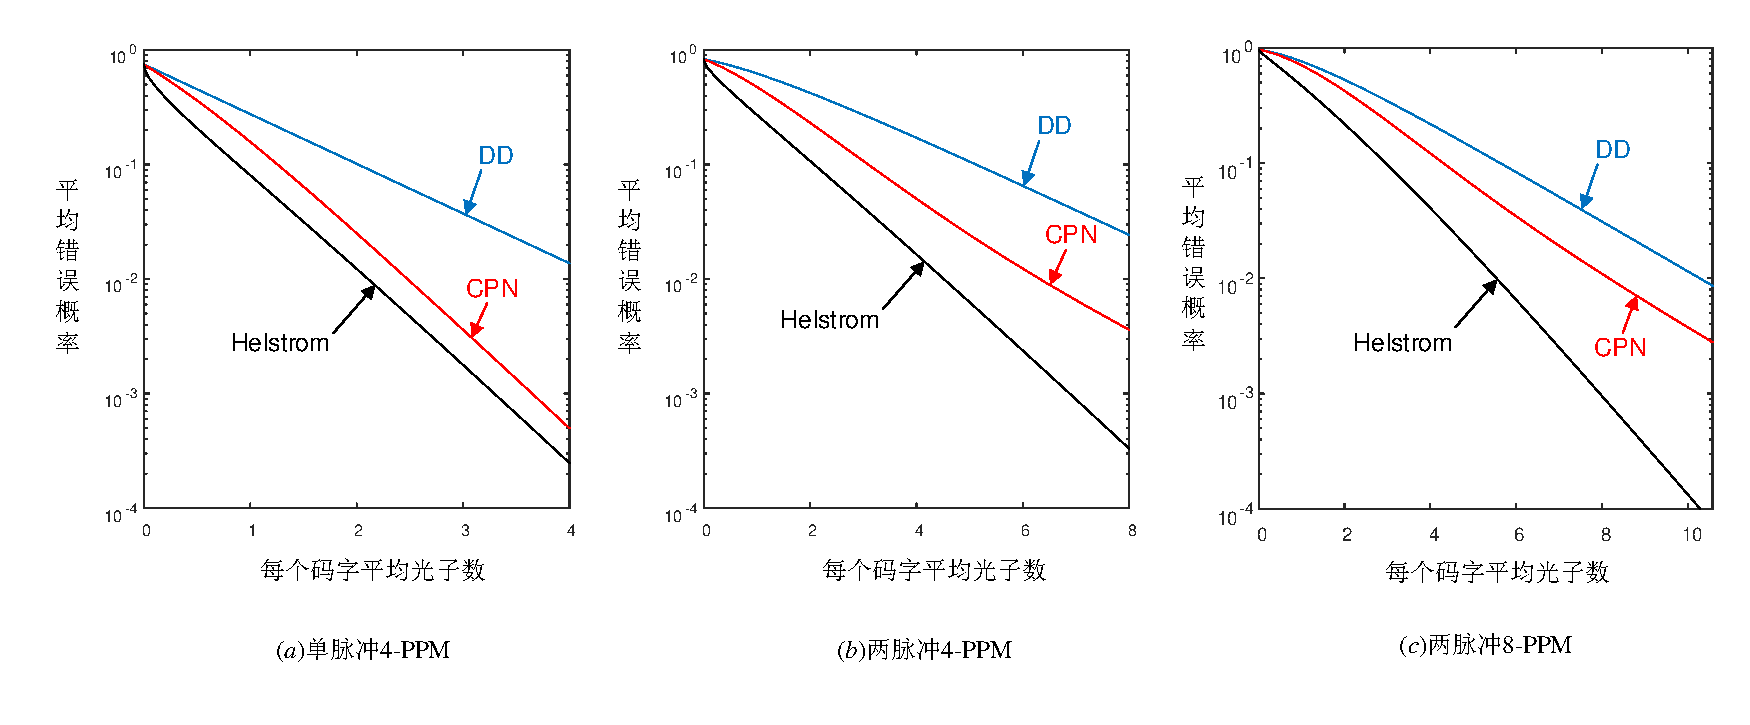
\includegraphics[width=\textwidth]{figures/chap4/4MPPM-error}
  \caption{4个时隙的MPPM性能曲线}
  \label{fig:4MPPM-error}
\end{figure}

\begin{figure}
\centering
  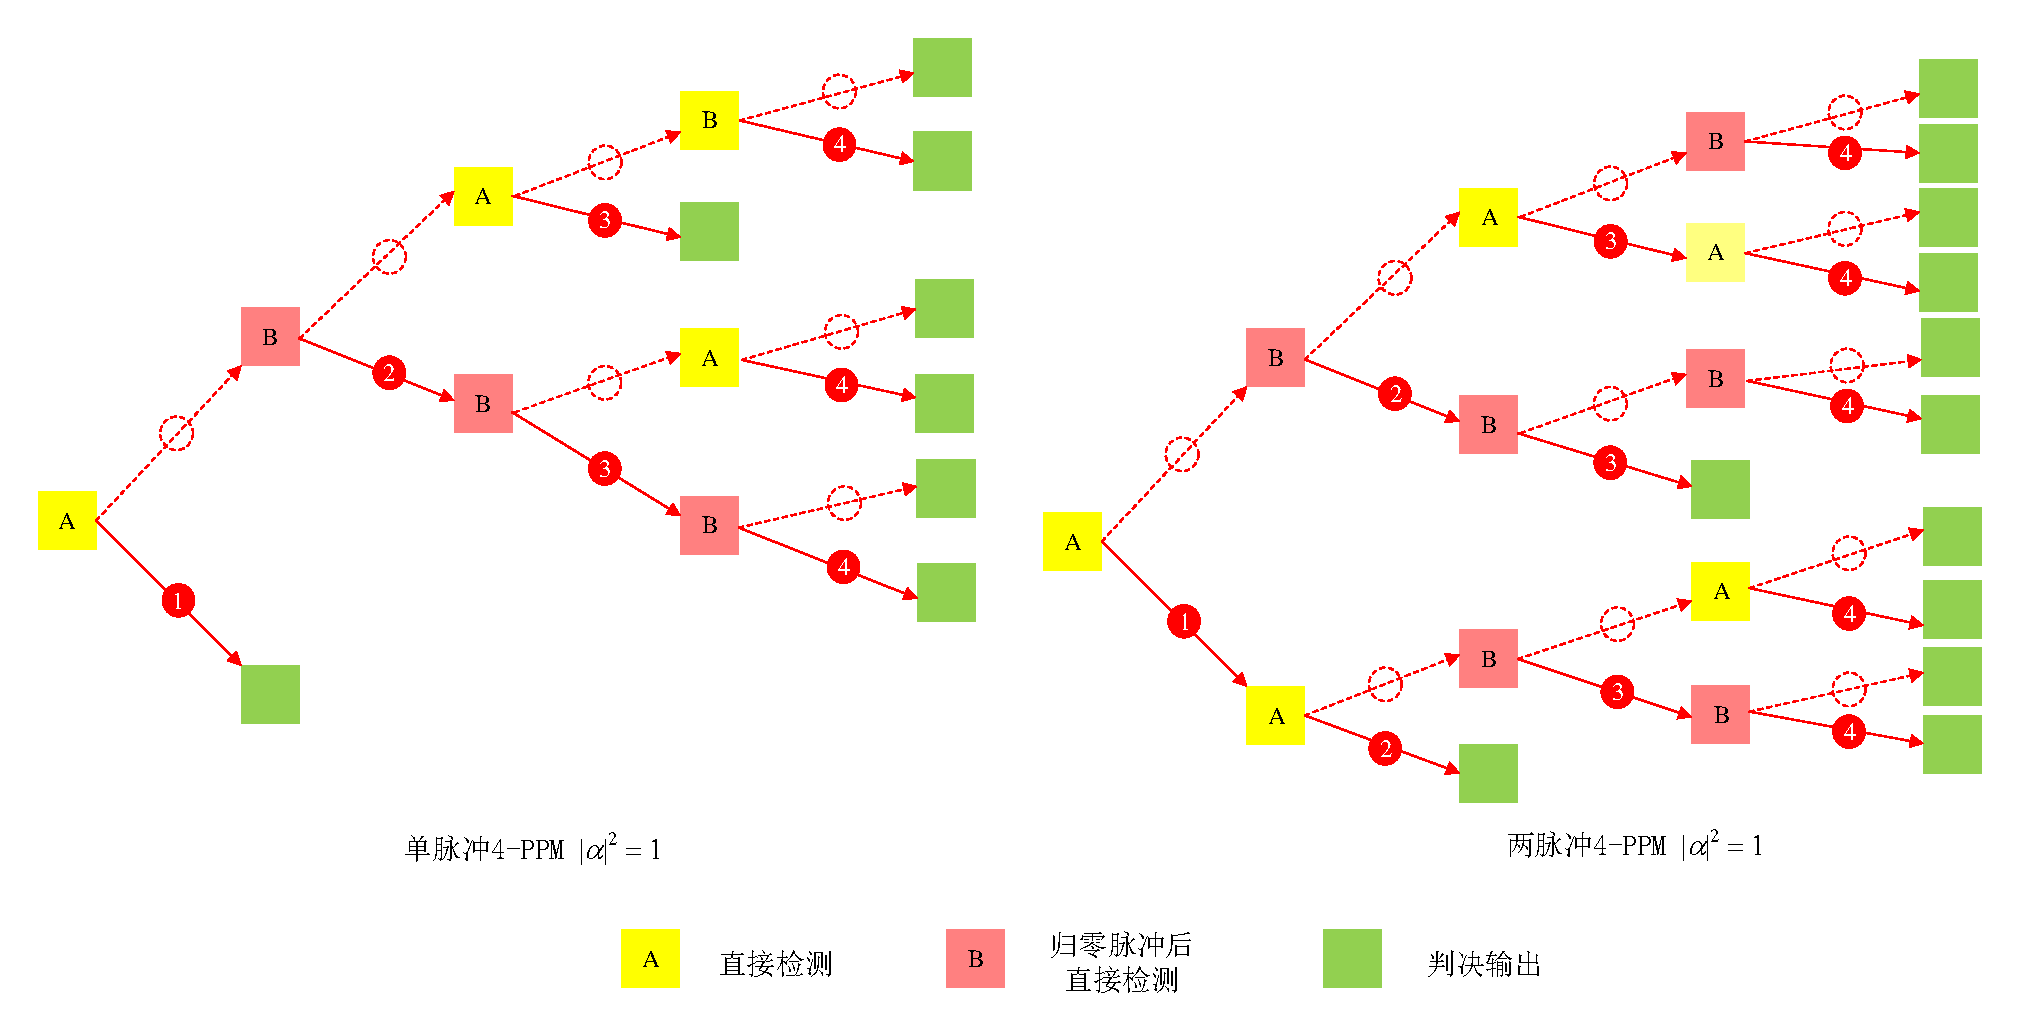
\includegraphics[width=\textwidth]{figures/chap4/2-4-PPM-DT}
  \caption{4个时隙的MPPM控制策略决策树}
  \label{fig:4MPPM-DT}
\end{figure}

利用上述算法,我们分别对4个时隙的单脉冲PPM、
4个时隙两脉冲PPM和8个时隙两脉冲PPM信号进行数值仿真计算,
仿真结果如图\ref{fig:4MPPM-error}所示。
对于单脉冲情况下,就是4-PPM信号,其中蓝色的线代表直接检测(DD)方案,
也就是标准量子极限,红色的线代表条件归零接收机(CPN),
黑色的线代表Helstrom量子极限,
经过对比发现,
虽然通过动态规划优化出来的策略与Dolinar的策略有所差异,
如图\ref{fig:4MPPM-DT}所示,
但是其性能与Dolinar的CPN接收机是相同的,
能够无条件的突破标准量子极限,
即在任意光子数下平均错误概率都比标准量子极限要低。
这表明,最优控制策略并不是唯一的,
而是存在多个最优控制策略。
对于两脉冲情况,从图\ref{fig:4MPPM-error}可以看到,
不论是2-4-PPM还是2-8-PPM信号,
最优控制策略下的条件归零接收机可以
无条件的突破标准量子极限。





\section{编码后二元调制信号条件归零接收机}
在上一小节中,我们讨论了MPPM信号,
它可以看做一种特殊的二进制编码信号,
在这一节里,我们来讨论对任意二进制编码信号,
采用最优控制策略的条件归零接收机,
能否突破传统检测方案的标准量子极限。

\subsection{Hamming码与极化编码}
首先我们来讨论两种重要的编码,
Hamming码和极化编码,以这两种编码为例,分析我们
这种采用最优控制策略的条件归零接收机的性能。

Hamming码是一种古老的编码方式,它是一类参数为
$(2^m-1, 2^m-1-m, m)$的二进制线性码\cite{jd2001xxlybm}。
它的生成矩阵为$G= [ I_k  | A^T]$,
其中$I_k$是$k=2^m-1-m$维单位矩阵,
$A^T$的每一行是是一个长度为$m$的非零二进制向量,
不能为单位向量且两两独立,这种向量一共
有$2^m-1-m$个,按照任意一种排列方式组合成矩阵$A^T$。
它对应的校验矩阵为$H = [A | I_{m}]$满足校验方程
$H G^T = 0$。一般的,我们称这种码字为[$2^m-1$, $2^m-1-m$]Hamming码。
例如[7, 4]Hamming码的生成矩阵为
\begin{equation}
G = \begin{bmatrix}
        1 & 0 & 0 & 0 & 1 & 1 & 0 \\
        0 & 1 & 0 & 0 & 1 & 0 & 1 \\
        0 & 0 & 1 & 0 & 0 & 1 & 1 \\
        0 & 0 & 0 & 1 & 1 & 1 & 1 
    \end{bmatrix}
\end{equation}
利用生成矩阵,我们可以得到所有的码字为
\begin{equation}
c_i = x_i G, i=0,1,...,2^m-1.
\end{equation}
其中$x_i$为数字$i$的$m$位二进制表达。

极化编码是一种利用信道极化特性设计的一种编码方案\cite{arikan2009channel,korada2009polar,wilde2013polar},
采用这种编码方案能够逼近Holevo容量\cite{guha2012polar}。
极化编码也可以看做一种特殊的Reed-Muller(RM)码,
可以通过如下方法生成\cite{arikan2008performance}。
首先生成n阶RM码的生成矩阵
\begin{equation}
G_{RM}(n, n) = F^{\otimes n}.
\end{equation}
其中
\begin{equation}
F = \begin{bmatrix}
        1 & 0 \\
        1 & 1  
    \end{bmatrix}
\end{equation}
$F^{\otimes n}$ 表示n阶张量积。
例如,$G_{RM}(3,3)$为
\begin{equation}
G_{RM}(3,3) = \left[
\begin{array}{cccccccc}
 1 & 0 & 0 & 0 & 0 & 0 & 0 & 0 \\
 1 & 1 & 0 & 0 & 0 & 0 & 0 & 0 \\
 1 & 0 & 1 & 0 & 0 & 0 & 0 & 0 \\
 1 & 1 & 1 & 1 & 0 & 0 & 0 & 0 \\
 1 & 0 & 0 & 0 & 1 & 0 & 0 & 0 \\
 1 & 1 & 0 & 0 & 1 & 1 & 0 & 0 \\
 1 & 0 & 1 & 0 & 1 & 0 & 1 & 0 \\
 1 & 1 & 1 & 1 & 1 & 1 & 1 & 1 \\
\end{array}
\right].
\end{equation}
极化编码只选取满足特定条件的行构成生成矩阵。
首先我们通过如下递归关系
计算极化率向量$z_N = (z_{N,1}, ..., z_{N,N})$
\begin{equation}
\begin{split}
z_{1,1} &= 1/2, \\
z_{2k, j} &= \begin{cases}
                2 z_{k,j} - z_{k,j}^2 & 1 \le j \le k, \\
                z_{k,j-k}^2           & k+1 \le j \le 2k .
            \end{cases}
\end{split}
\end{equation}
接着,我们构造$(1,...,N)$的一个排列$\pi_N = (i_1, ..., i_N)$,
使得在此排列下,极化向量$z_N$是递减的。
那么,对于任意$N=2^n$,$1 \le K \le N$,
[N,K]极化编码矩阵$G_P(N,K)$是由$G_{RM}(n,n)$中
行数在$(i_1,i_2,...,i_K)$中的行构成的子阵。
例如$n=3,K=5$时,极化向量前5个元素对应的下标为
$(8, 4, 6, 7, 2)$,所以
\begin{equation}
G_{P}(8,5) = \left[
\begin{array}{cccccccc}
 1 & 1 & 0 & 0 & 0 & 0 & 0 & 0 \\
 1 & 1 & 1 & 1 & 0 & 0 & 0 & 0 \\
 1 & 1 & 0 & 0 & 1 & 1 & 0 & 0 \\
 1 & 0 & 1 & 0 & 1 & 0 & 1 & 0 \\
 1 & 1 & 1 & 1 & 1 & 1 & 1 & 1 \\
\end{array}
\right].
\end{equation}


\subsection{编码后二元调制信号标准量子极限}
在经典检测方案中,符号探测与译码是两个独立的过程,
因此对编码后的二元调制信号,探测也是通过直接探测每一个时隙进行的,
最后采用最大似然译码准则进行译码。
对于OOK调制,设符号集合为$\{\ket{0}, \ket{\alpha}\}$,这一章$\alpha$都取实数,
在每一个时隙里面,与MPPM一样采用直接探测,可以用式\ref{eq:ONOFF-POVM} 的二元POVM测量表示,
其对应的条件概率由式\ref{eq:CPN-cond-1}给出。
而对BPSK调制,设符号集合为$\{\ket{-\alpha}, \ket{\alpha}\}$,
在每一个时隙里面,采用的是零差接收方式,对应于二元POVM测量
\begin{equation}
\begin{split}
\hat{\Pi}_0 &= \int_{-\infty}^0 \ket{x}\bra{x} dx, \\
\hat{\Pi}_1 &= \int_0^{\infty} \ket{x}\bra{x} dx.
\end{split}
\end{equation}
而条件概率为
\begin{equation}
\begin{split}
p_{0|0} &= \int_{-\infty}^0 |\bra{x}\ket{-\alpha}|^2 dx = \frac{1}{2}(1+\erf{\sqrt{2}\alpha}) \\
p_{1|1} &= \int_0^{\infty} |\bra{x}\ket{\alpha}|^2 dx = \frac{1}{2}(1+\erf{\sqrt{2}\alpha}) 
\end{split}
\end{equation}
这里用0表示符号$\ket{-\alpha}$,而用1表示符号$\ket{\alpha}$,
用$p_{0|0}$和$p_{1|1}$分别表示在符号0和符号1的情况下,探测正确的概率。
在大信号近似下,利用余误差函数的CHernoff界\cite{chang2011chernoff},可得
\begin{equation}
p_{0|0} = p_{1|1} = 1 - \frac{1}{2} e^{-2\alpha^2}.
\end{equation}
因此对应的平均错误概率为
\begin{equation}
p_e \approx \frac{1}{2} e^{-2\alpha^2}.
\end{equation}

对一般的编码信号,
精确地分析误符号率十分困难,
但是可以采用上一章动态规划的方法,
设置控制参数都为0,
就可以得到精确的数值结果。
为了便于进一步分析,这里我们采用近似分析,
只考虑在大信号近似的情况下,即$|\alpha| \gg 1$时,
接收机的误符号率。
我们假设码字的最小汉明距离为$d_{\min}$,
那么在一个码字内,
发生$f = \lceil d_{\min}/2 \rceil$个比特错误
将无法通过译码纠错,
它的概率近似为 $Ae^{-f n}$,其中$A$为某个常数,参数
\begin{equation}
n = \begin{cases}
        |\alpha|^2 & OOK, \\
        2|\alpha|^2 & BPSK.
    \end{cases}
\end{equation}
因为发生更多比特错误的概率是它的高阶小量,可以忽略,
所以经典的探测方案大信号近似下,
平均错误概率$\sim e^{-\lceil d_{\min}/2\rceil n}$,
例如,(7,4)Hamming码的最小汉明距离为3,
所以它的误符号率$\sim e^{-2n}$。
而(8,5)极化码最小汉明距离为2,所以
它的误符号率$\sim e^{-n}$。


\subsection{编码后二元调制信号最优量子检测极限}
根据上一节的分析,我们知道对一个码符号集合,
只要得到符号集合的Gram矩阵,
就可以利用最优量子检测的极限可以通过半正定规划的方法
得到精确。对于任意编码的二元调制信号,Gram矩阵都可以写为
\begin{equation}
G_{i,j} = e^{1/2 d(c_i, c_j) n}.
\end{equation}
其中$c_i$是第$i$个码字,$d(c_i, c_j)$是两个码字的汉明距离,
参数$n$如前面的定义。
根据Gram矩阵,就可以利用CVX工具箱\cite{cvx,gb08}求解问题\ref{eq:Hel-SDP}
得到最优解了。

为了方便分析,我们也采用大信号近似,根据前面的结论,
大信号时的平均错误概率$\sim e^{-d_{\min} n}$,
这里$d_{\min}$为码字的最小汉明距离。





\subsection{编码后二元调制信号条件归零接收机}
对于编码后的二元调制信号,包括OOK调制和BPSK调制,
我们采用与MPPM相似的接收机结构,
只是接收策略不同。

与MPPM信号类似,编码后的OOK信号在每一个时隙里面的
测量策略是一样的,都是从直接检测和归零脉冲后再直接检测
这两种测量方案中,根据历史输出和优化策略选择一种进行探测。
而对于BPSK调制,则有所不同。
在每一个时隙里面,编码后的BPSK调制条件归零接收机在
两种Kennedy接收机中选择一个进行探测。


\begin{figure}
\centering
  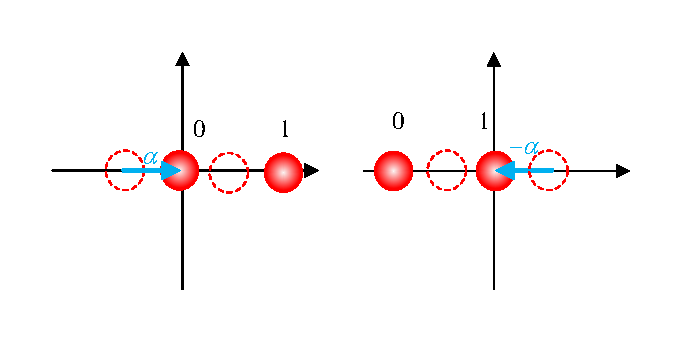
\includegraphics[height=5cm]{figures/chap4/BSPK-AB-receiver}
  \caption{在每个时隙中BPSK调制采用的两种Kennedy接收方案}
  \label{fig:BSPK-AB-receiver}
\end{figure}





如图\ref{fig:BSPK-AB-receiver}所示,
第一种Kennedy接收机通过一个位移操作$\hat{D}(\alpha)$,
将BPSK符号集合变成OOK调制$\{\ket{0}, \ket{2\alpha}\}$
然后直接探测,它对应于二元POVM测量
\begin{equation}
\begin{split}
\Pi_0 &= \hat{D}(\alpha)^\dagger \ket{0}\bra{0} \hat{D}(\alpha) ,\\
\Pi_1 &= \hat{D}(\alpha)^\dagger (\hat{I} - \ket{0}\bra{0}) \hat{D}(\alpha) .
\end{split}
\end{equation}
在这组POVM测量下,探测的条件概率为
\begin{equation}
\begin{split}
p_{0|0} &= 1, \\
p_{1|1} &= 1 - e^{-4|\alpha|^2}.
\end{split}
\end{equation}
这里我们用$p_{0|0}$表示在信号0的情况下,
输出为0,即没有光子计数发生,
而$p_{1|1}$表示在信号1的情况下,
输出为1,即发生了光子计数事件。
第二种Kennedy接收机通过一个位移操作$\hat{D}(-\alpha)$,
将BPSK符号集合变成$\{ \ket{-2\alpha}, \ket{0}\}$
然后直接探测,它对应于二元POVM测量
\begin{equation}
\begin{split}
\Pi_0 &= \hat{D}(-\alpha)^\dagger \ket{0}\bra{0} \hat{D}(-\alpha) ,\\
\Pi_1 &= \hat{D}(-\alpha)^\dagger (\hat{I} - \ket{0}\bra{0}) \hat{D}(-\alpha) .
\end{split}
\end{equation}
在这组POVM测量下,探测的条件概率为
\begin{equation}
\begin{split}
p_{0|0} &= e^{-4|\alpha|^2}, \\
p_{1|1} &= 0.
\end{split}
\end{equation}

\begin{figure}[H]
\centering
  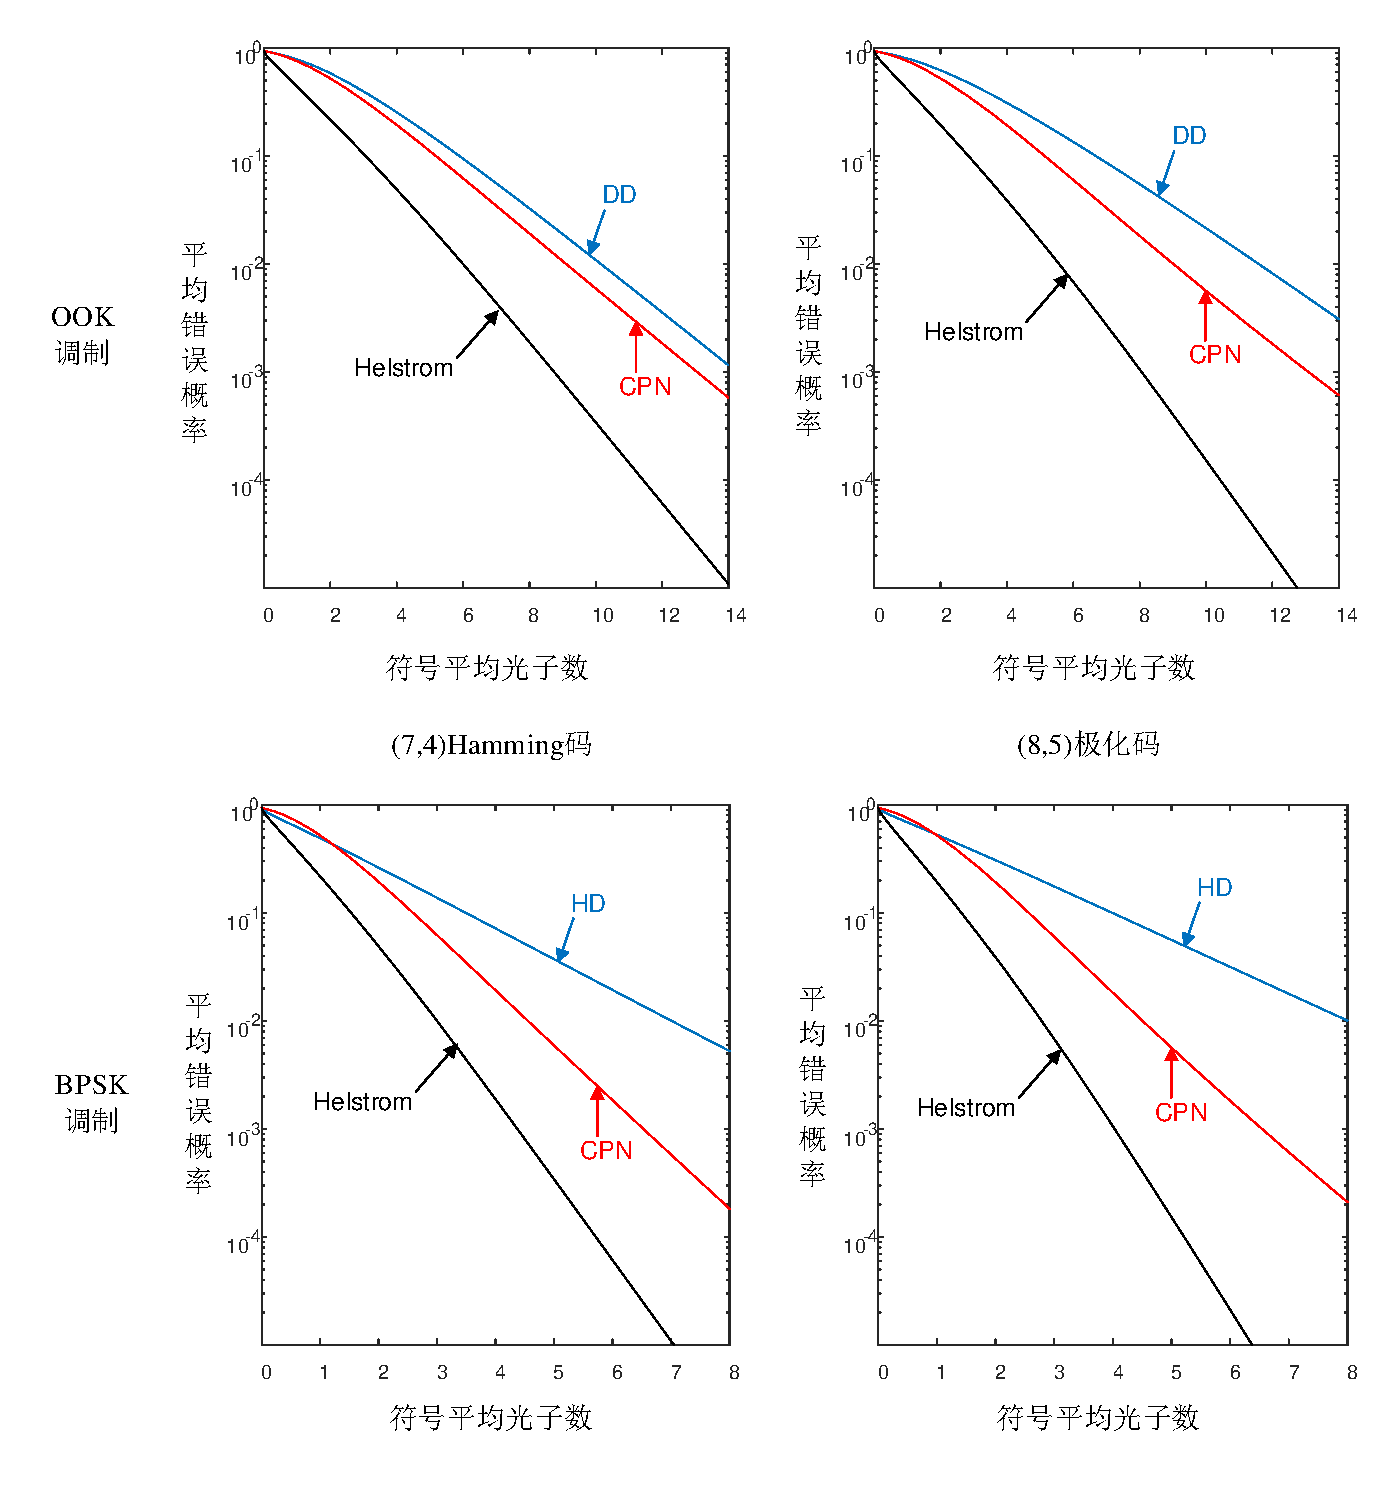
\includegraphics[width=\textwidth]{figures/chap4/OOK-Code-error}
  \caption{OOK信号汉明码和极化码的条件归零接收机性能}
  \label{fig:OOK-Code-error}
\end{figure}


利用上述结果,我们就可以利用式\ref{eq:state-transform}更新状态方程了,
进而采用动态规划的方法对控制策略进行优化。
我们选择了(7,4)汉明码和(8,4)极化码进行数值仿真,
仿真结果如图\ref{fig:OOK-Code-error}所示。
可以看到,对于OOK调制这两种不同的编码方案,
条件归零接收机可以在任意光子数下突破经典检测的极限。
当每个符号的平均光子数为14时,因为每一个Hamming码
码字平均有3.5个脉冲,因此每个脉冲的平均光子数为4,
此时采用条件归零接收机可以有近3dB的收益。
对于极化码,当每个符号的平均光子数为14时,
因为每一个极化码
码字平均有4个脉冲,因此每个脉冲的平均光子数为3.5,
此时采用条件归零接收机有7.4dB的收益。
对于BPSK调制这两种不同的编码方案,
可以看到条件归零接收机在信号较大时才能突破经典检测的极限,
而在码字信号平均光子数小于1时,
这种接收方案反而会比零差接收机要差。
但是当光子数增大时,这种接收方案比经典接收方案的收益
随着显著增大。
对比OOK和BPSK两种调制,可以发现要达到相同的误码率,
在相同的编码情况下,采用BPSK调制的条件归零接收机所需要的
能量更低,因而具有更高的能量效率。

